%!TEX root = ../thesis.tex
%*******************************************************************************
%***************************** Fifth Chapter **********************************
%*******************************************************************************
\graphicspath{{Chapter5/Figs/Vector/}{Chapter5/Figs/}}

%%%%%%%%%%%%%%%%%%%%%%%%%%%%%%%%%%%%%%%%%%%%%%%%%%%%%%%%%%%%%%%%%%%%%%%%%%%%%%%%
% The Portal
%%%%%%%%%%%%%%%%%%%%%%%%%%%%%%%%%%%%%%%%%%%%%%%%%%%%%%%%%%%%%%%%%%%%%%%%%%%%%%%%
% - Is it possible to communicate the inner workings of the system through the
%   user interface?
% #region
\chapter{The Portal}
\section{Introduction}
The term 'reasoning' in the title, meaning "the action of thinking about something in a logical, sensible way", may have been redundant if a system were to calculate trip prices autonomously. But this system is designed with the user in mind. That is why the inner workings of the system must be expressed in such a way that allows the user to predict the outcome after changes have been made to pricing rules with confidence.
% #endregion

%%%%%%%%%%%%%%%%%%%%%%%%%%%%%%%%%%%%%%%%%%%%%%%%%%%%%%%%%%%%%%%%%%%%%%%%%%%%%%%%
% Visual Hierarchy
%%%%%%%%%%%%%%%%%%%%%%%%%%%%%%%%%%%%%%%%%%%%%%%%%%%%%%%%%%%%%%%%%%%%%%%%%%%%%%%%
% #region
\section{Visual Hierarchy}
A pricing rule is a set of criteria that covers pricing information. These criteria and pricing information are stored in database entities. These entities could be expressed as view components. For example, "the pickup location of a trip must be located in Amsterdam" is a criterion that is stored in a location entity, that may be expressed as polygon on a world map component.

\subsection{Essential Components}
The main entities that make up a the price calculation system are visualized in Figure \ref{fig:Treemap}. The plurality of the child entities describe whether more than one child are present within the parent entity. For example, rules have many products, with each product having one price, which has one priceFixed and one priceDynamic.

\begin{figure}[H]
	\centering
	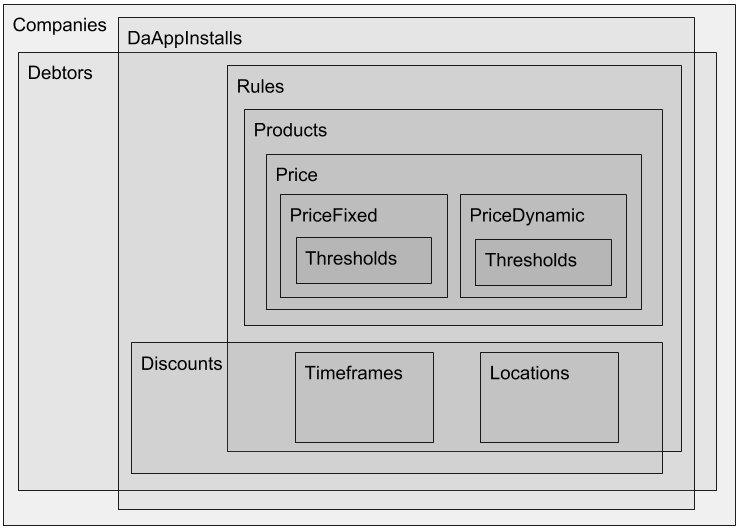
\includegraphics[width=0.7\textwidth]{Treemap}
	\caption[Treemap of Components]{Treemap of entities.}
	\label{fig:Treemap}
\end{figure}

\subsection{Expressing Order}
A human brain is capable of ordering the differently sized boxes by enclosure, proximity, intensity, and spatial grouping. Stephen Few states that "Perception of these basic visual attributes is called 'preattentive' processing, in contrast to the conscious part of perception, which is called 'attentive' processing. Preattentive processing is extremely fast and broadband in that we can simultaneously perceive a large number of these basic visual attributes, called 'preattentive attributes'. Preattentive perception is done in parallel, but attentive processing is done serially and is, therefore, much slower." in \cite[p.~3]{few}. This fact can be utilized to construct a hierarchy similar to that of Figure \ref{fig:Treemap} through visual queues. A famous phrase often used in data visualizations called Shneiderman's mantra \cite{mantra}, lays the foundation of principles that enable users to maintain an understanding of the context in which data is visualized. The sentences in the mantra dictate that there are three stages in data exploration. This mantra in combination with preattentive attributes could be put to good use in reducing the cognitive overhead while reasoning about pricing rules.

\begin{enumerate}
	\item Overview First
	\item Zoom and Filter
	\item Details on Demand
\end{enumerate}
% #endregion

%%%%%%%%%%%%%%%%%%%%%%%%%%%%%%%%%%%%%%%%%%%%%%%%%%%%%%%%%%%%%%%%%%%%%%%%%%%%%%%%
% Design
%%%%%%%%%%%%%%%%%%%%%%%%%%%%%%%%%%%%%%%%%%%%%%%%%%%%%%%%%%%%%%%%%%%%%%%%%%%%%%%%
% #region
\section{Design}
% Which backend concepts are essential to display in the frontend?
Composing a pricing rule should require no level of cognitive effort. It should be linear process where few choices result in the desired outcome. This could be achieved by separating related reusable entity components from the pricing rule. For example, a location does not have to be defined in the pricing rule view. It could be defined in its own separate view, so that it can later be selected, allowing the user to only reason about a subset of criteria at once. This theory works for reusable entities such as locations, but would result in a negative outcome when used with information that belongs to a single pricing rule, such as dynamic or fixed prices. The contextual understanding is lost when the user has navigate to a different view, while keeping locations, time, rule type, and other properties in memory while filling in the different price properties for different products. The mantra could be applied to offer an overview of a particular entity. The user could then select an entity and modify the details. Displaying the properties on a single page, ordered using preattentive attributes. The portal follows a basic hierarchy:

\begin{enumerate}
	\item Overview: enumerates over a list of entities
	\item Detail page: contains one particular entity
	\item Composite page: displays a combination of lists of entities and/or single entities that belong together
\end{enumerate}

Entities that are part of a many-to-many or one-to-many relation should have their own overview and detail pages, otherwise the user may think that a particular entity that is combined into another entity's view, may exist for that entity only. If the user modifies that entity, it has consequences for all other relationships with that entity. For example, if a location was shared between many rules, the user could edit the address of the location, unaware of the consequences that the change brings to all the rules that depend on that particular location. One-to-one or many-to-one relationships do not have that problem. For example, thresholds are embedded, meaning that they are not part of any entity other than the one that embeds them. With this concept, the following entities should have their own overview and detail pages: Products, Locations, Rules, Discounts, and DaAppInstalls. The mantra could also be applied to the representation of entity properties in the same fashion. But for each enumeration, a direction of space on the page must be filled. As a webpage only has two dimensions of space, the properties that fill up the space must be grouped in some fashion. Preattentive attributes can be utilized to illustrate that some elements on composite pages belong to each other, or are in fact distinct.
% #endregion

%%%%%%%%%%%%%%%%%%%%%%%%%%%%%%%%%%%%%%%%%%%%%%%%%%%%%%%%%%%%%%%%%%%%%%%%%%%%%%%%
% Products
%%%%%%%%%%%%%%%%%%%%%%%%%%%%%%%%%%%%%%%%%%%%%%%%%%%%%%%%%%%%%%%%%%%%%%%%%%%%%%%%
% #region
\section{Products}
The sidebar contains links to the overview pages. The products overview page shows a searchable and sortable list of products. These products may be selected, upon which the user is brought to the detail page where the type, name and other properties can be set, and where the product may be deleted. When properties have changed, the save button becomes available. And when the user tries to leave the page after changing a property, a prompt is shown that allows the user to leave or continue editing a product. These features have been implemented for all components.
% #endregion

%%%%%%%%%%%%%%%%%%%%%%%%%%%%%%%%%%%%%%%%%%%%%%%%%%%%%%%%%%%%%%%%%%%%%%%%%%%%%%%%
% Pricing
%%%%%%%%%%%%%%%%%%%%%%%%%%%%%%%%%%%%%%%%%%%%%%%%%%%%%%%%%%%%%%%%%%%%%%%%%%%%%%%%
% #region
\section{Pricing}
The pricing overview contains a table with two tabs: 'rules' and 'special rates'. The word 'discounts' may imply that it would only be able to lower the prices of trips. Special rates can be negative or positive, and can be expressed in percentages or fixed amounts. Discounts and rules have a lot in common. They both have locations and timeframes, they can both be prioritized, and they both have an impact on price calculations.

\subsection{Discounts}
On the discount detail page, the name, priority, type and value properties may be set. The discount type can be changed between 'fixed' and 'percentage', changing the symbol next to the value from a \euro to a \% symbol. The timeframes and locations can be found below the normal properties. For the timeframes a component has been created that can be integrated into any form. Timeframes consist of two dates between which a discount or rule is active. A date picker allows users specify the date, and a separate time input allows users to specify the time. When users want to define more complex timeframes, a specific week days option opens up an hour selection element. When this option is enabled, the time inputs are hidden. Only one option can be enabled so that no confusion between the time aspect of the timeframes can exist. When this toggle is set, the time aspect of the start and end date is hidden, as from that moment, time can only be defined as individual hours. Because this aspect of the timeframe is stored as a bit string, it is easily translated into an html input element, and can easily be modified in the future. The location selector component can be found right above the timeframe selector component. It has a 'from' and a 'to' input in which the user may enter a location by name or address. Autocompletion results allow the user to quickly find a one of the company defined locations. When the user presses enter and the location does not exist, the user is prompted to create a new location. All locations that have been created by developers may be shared, so that the user is able to clone them. This is added as a requirement in a later stage, allowing users to create pricing rules without having to bother with locations first. When the input is empty, the 'Everywhere' option is selected, which ensures that no location is associated with that input.

\subsection{Rules}
On top of the functionalities just covered, the rule detail page has more complex property inputs. A table of columns for each product is displayed with a minimum price, waiting price, start price, kilometer price, and minute price inputs on each row. The kilometer and minute price can be extended through thresholds. When a threshold is added, it copies the values from the row above, which may then be edited. The timeframes and location selectors look the same as those of the discounts, but only when the rule is of type 'dynamic'. When the user selects the 'fixed' type, the form is transformed. The columns in the table only contain a waiting price and fixed price input. The location input is moved next to the fixed price input. The locations can no longer be set to 'Everywhere' to avoid expensive mistakes. A button allows prices to be extended with subrules, just like the way kilometer and minute prices could be extended with thresholds. A visual hierarchy exists between the different components on the page through proximity and spacial grouping. The views can be seen in Appendix \ref{appendix:slides_7}.

\subsection{Priority}
The priority for discounts and rules can be defined in the priority input field, although modifying this field would be inconvenient for large amounts of modifications. A drag and drop feature was added to sort more quickly.
% #endregion

%%%%%%%%%%%%%%%%%%%%%%%%%%%%%%%%%%%%%%%%%%%%%%%%%%%%%%%%%%%%%%%%%%%%%%%%%%%%%%%%
% Locations
%%%%%%%%%%%%%%%%%%%%%%%%%%%%%%%%%%%%%%%%%%%%%%%%%%%%%%%%%%%%%%%%%%%%%%%%%%%%%%%%
% #region
\section{Locations}
Locations have been defined as either points or areas. In technical terms, this is sound. For an average user, this does not sound intuitive. That is why locations are named as two groups: locations and areas. The technical solution in matching points was initially based on points being distinct coordinate pairs, which could only be precisely matched if the user selected a location from the location service that was never changed, like Google Places. The locations found in searches would exactly match the coordinate pairs, as that is where the points are originated from. But when a passenger drops a pin on the map, it would have very little to no chance of matching the exact coordinate pair. That is why all locations are stored as polygons initially, with a coordinate pair denoting the centroid of the location. The polygons may be imported, drawn and edited by the user in a later stage.

\begin{figure}[H]
	\centering
	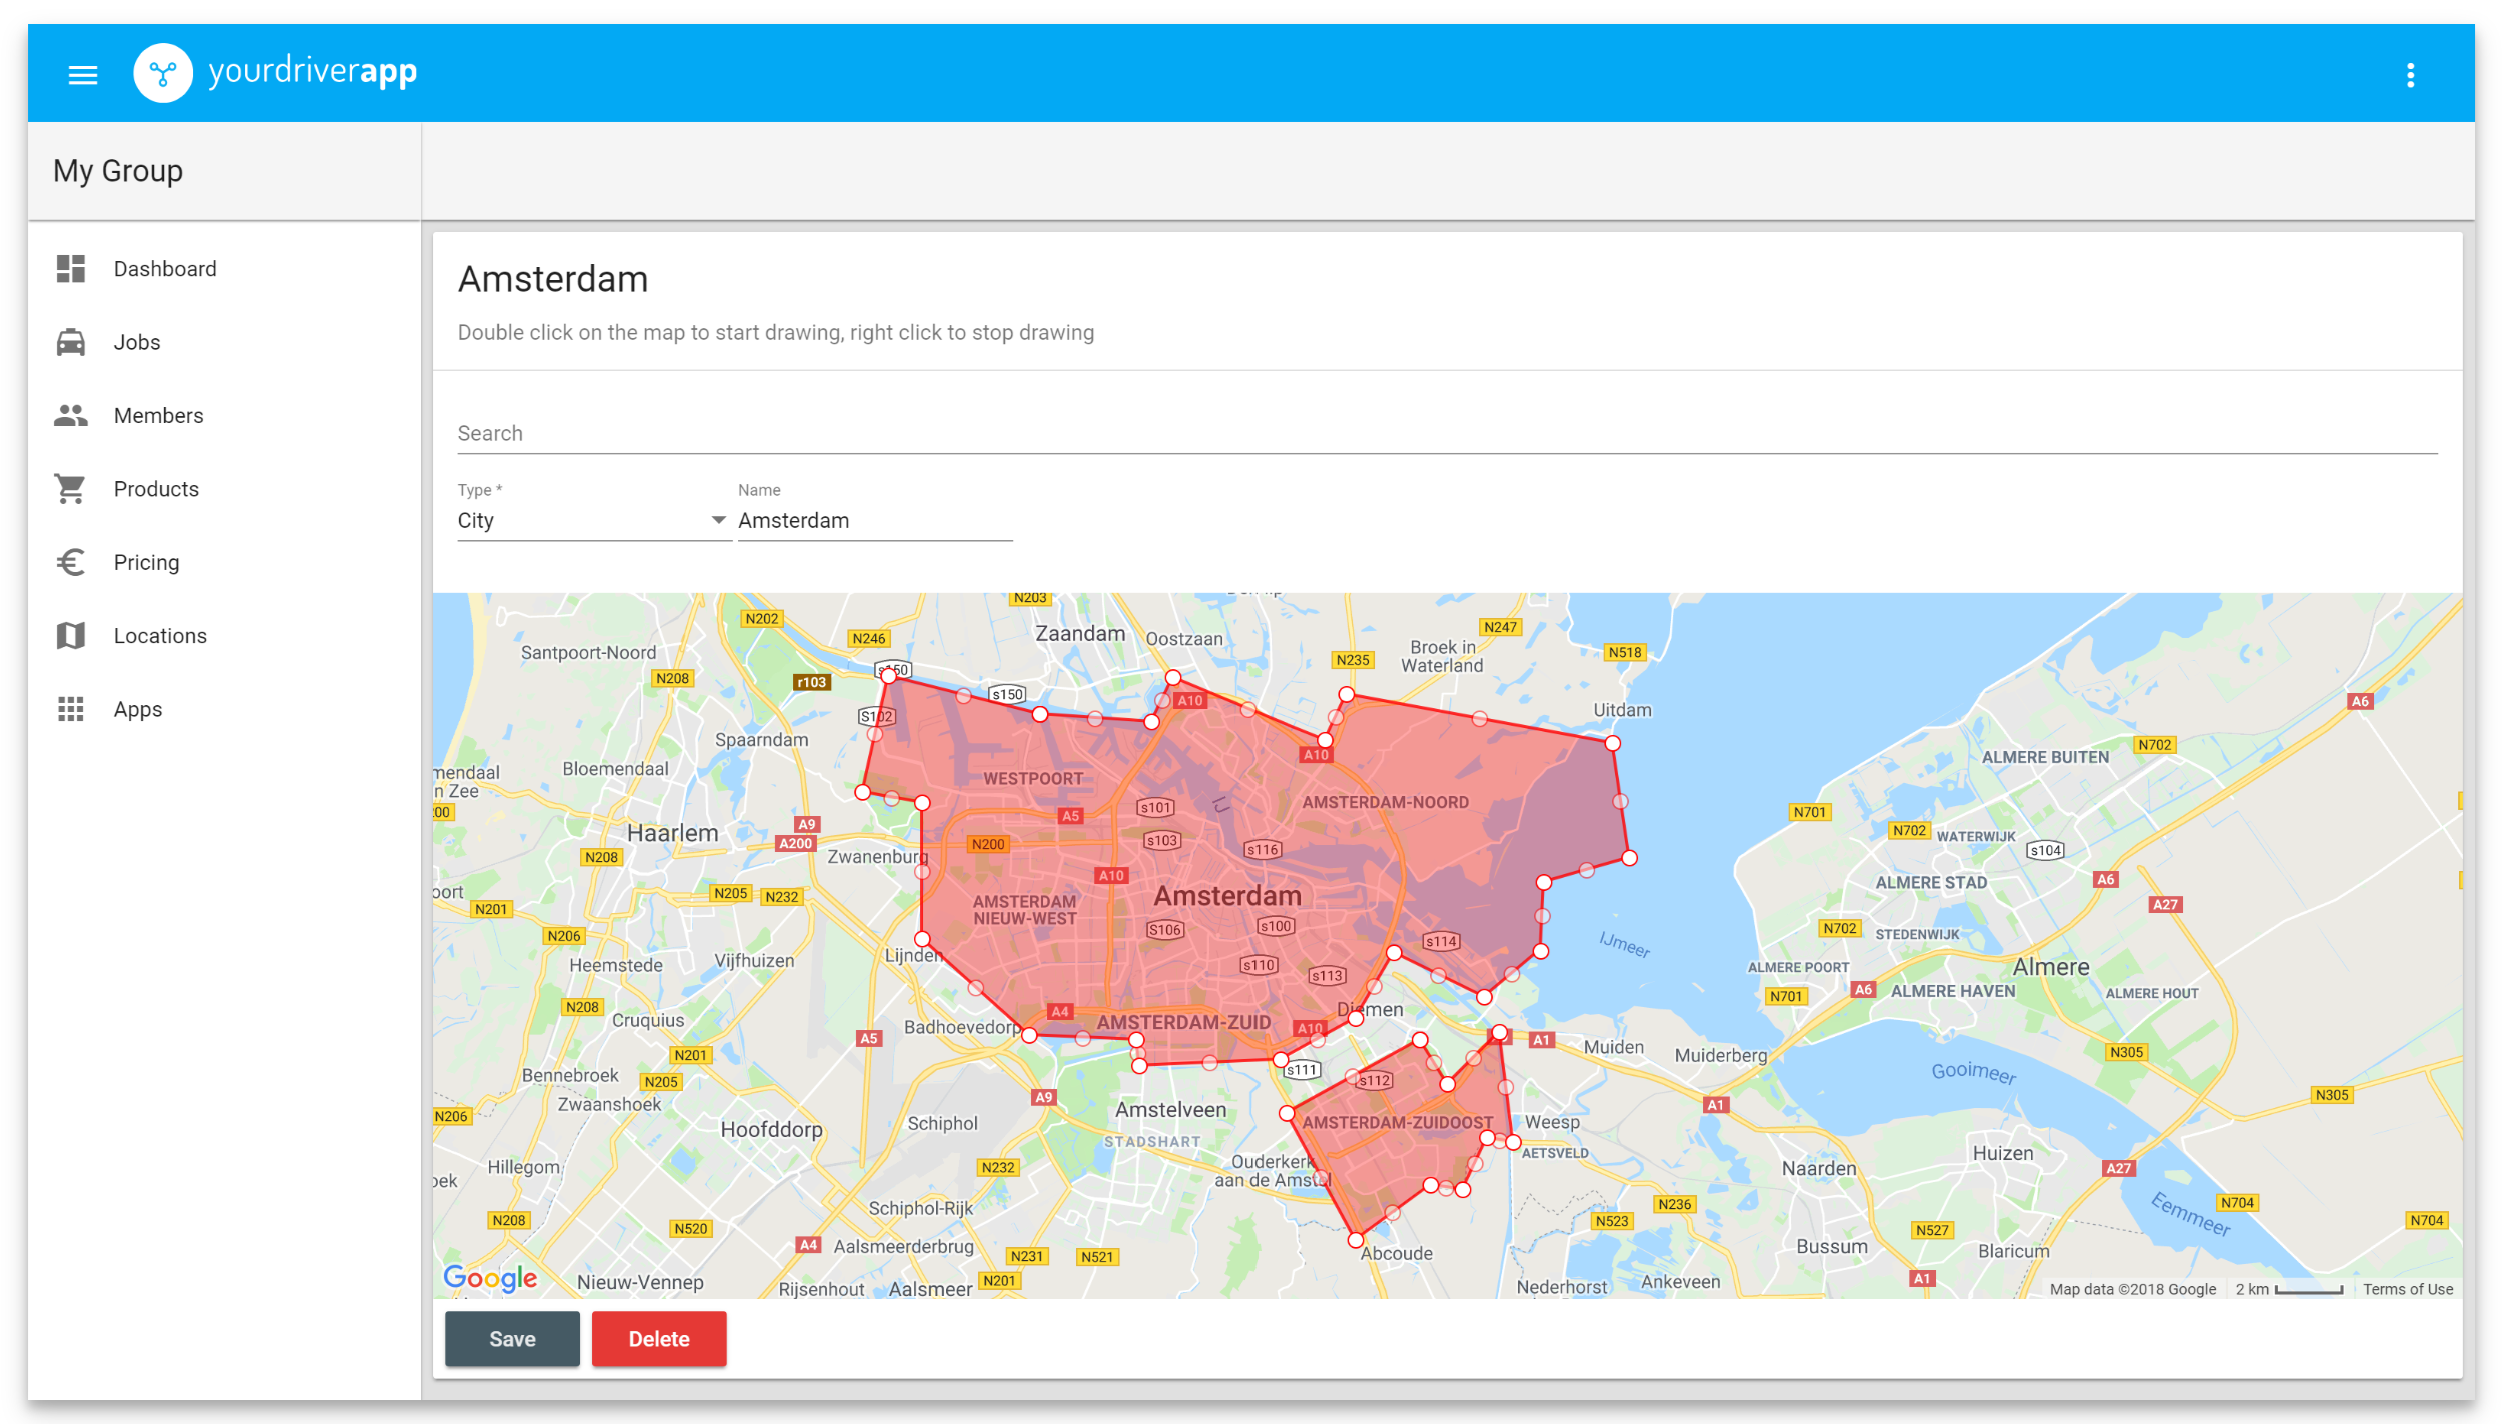
\includegraphics[width=0.9\textwidth]{AmsterdamShadow}
	\caption[Amsterdam Drawn Polygon]{Amsterdam - A single area comprised of multiple locations.}
	\label{fig:Amsterdam Drawn Polygon}
\end{figure}

\subsection{Point}
When a point is created, only a search bar is visible initially. Autocomplete suggestions from Google Places are shown when the user starts typing. These results are filtered to only include addresses and smaller locations, to maintain the distinction between areas and points. A shape class has been created that is capable of plotting points, polygons and multipolygons on a Google Map using a method called autoDetect. When the user selects a location, the gps coordinates are used as a center around which a polygon is plotted.

\begin{center}
\noindent\begin{minipage}{.85\textwidth}
\begin{lstlisting}[caption={Generating Polygon From Point.}, label={lst:Generating Polygon From Point}]
/**
 * Generate a polygon around lat lng coordinates.
 */
private static fromPoint(
	lat: number,
	lng: number,
	theta: number,
	radius: number,
) {
	const points = [];
	const p = (lat, lng, x, y, r) =>
		[lat + (r * x), lng + (r * y) * 1.5];

	let x, y;
	let angle = 0.0;

	while (angle < 2 * Math.PI) {
		x = length * Math.cos(angle);
		y = length * Math.sin(angle);
		points.push(p(lat, lng, x, y, radius));
		angle += Math.abs(theta);
	}

	// Closing the polygon.
	points.push(points[0]);
	return Shape.fromPolygon(points);
}
\end{lstlisting}
\end{minipage}
\end{center}

When a point is created, a user searches for a place in Google Places, gives it a name and a descriptor, and saves it as if it were a string of characters that would be matched within the system. After a point has been created, it may be modified by dragging the indices of the polygon. New polygons can be added by double clicking on the map, and edit mode can be stopped by right clicking on the map.

\subsection{Area}
The area detail page contains a map right at the creation screen. A search bar allows users to find a location, and add it to the map. The user may draw and modify polygons before the location is saved. The biggest difference between locations and areas is the search service that powers the autocomplete search. When a location is selected in the area search, a polygon is imported from OpenStreetMap as seen in Appendix \ref{appendix:slides_6}. Although this feature is great because it gives users the choice to avoid drawing polygons all together. The browser will have a hard time rendering all the indices of such complex shapes.
% #endregion

%%%%%%%%%%%%%%%%%%%%%%%%%%%%%%%%%%%%%%%%%%%%%%%%%%%%%%%%%%%%%%%%%%%%%%%%%%%%%%%%
% Apps
%%%%%%%%%%%%%%%%%%%%%%%%%%%%%%%%%%%%%%%%%%%%%%%%%%%%%%%%%%%%%%%%%%%%%%%%%%%%%%%%
% #region
\section{Apps}
After the user has created locations, products, special rates and rules, nothing will happen. When a new rule or discount is saved, it is not activated by default. The app detail page allows rules and discounts to be associated with an application, upon which they become active. For pricing rules, extra settings may be set that allow applications to show price estimations, or calculate the trip price using a taxi meter. From that point, the user is able to order a ride using the companies' booking app to test whether the expected outcome is the consequence of the changes.
% #endregion

\section{Conclusion on The Portal}
\[\textit{Is it possible to communicate the inner workings of the system through the user interface?}\]\hfill
The sidebar reflects which major concepts exist within the portal: Products, Pricing, Locations, and Apps. Composite views reflect the coherence that exists between related entities, while separation of independent entities reduce the cognitive overhead while reasoning about pricing rules. Spatial grouping on the page hint which properties belong to which entity, for which all human beings have a natural intuition. Manual activation and sorting of rules force the user to actively decide whether a rule should match, which can be tested immediately using the companies' booking app.
% essential concepts